%\documentclass[12pt,handout]{beamer}
\documentclass{beamer}
\usepackage[ngerman]{babel}
\usepackage[utf8]{inputenc}
\usepackage{amsmath}
\usepackage{amssymb}
\usepackage{listings} 
\usepackage{stmaryrd}
\lstset{language=Python, tabsize=4, showstringspaces=false,basicstyle=\footnotesize,mathescape=true}
\lstset{literate=%
  {Ö}{{\"O}}1
  {Ä}{{\"A}}1
  {Ü}{{\"U}}1
  {ß}{{\ss}}1
  {ü}{{\"u}}1
  {ä}{{\"a}}1
  {ö}{{\"o}}1
}
\usepackage{mathtools}
\usepackage{ulem}
\usepackage{tikz}

\usetheme{Boadilla}
\mode<presentation>{
\useoutertheme[subsection=false]{miniframes}
\useinnertheme{rectangles}
%\usecolortheme{crane}
}
\parskip 10pt

\begin{document}
\title{Informatik}   
\author{Abstrakte Datentypen - Baum} 
\date{}
\frame{\titlepage} 

%---
\begin{frame}[fragile]

Ein \textit{binärer Baum} ist entweder leer oder besteht aus einem Knoten, dem zwei binäre Bäume zugeordnet sind. 

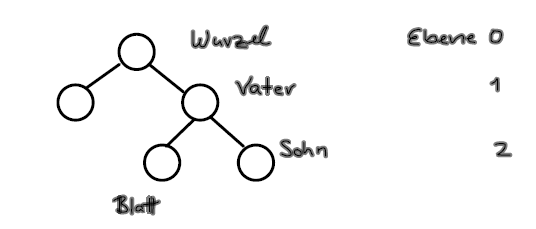
\includegraphics[scale=0.8]{bild1.png}
\end{frame}

%---
\begin{frame}[fragile]

In den Knoten eines Baums können beliebige Objekte gespeichert werden.  

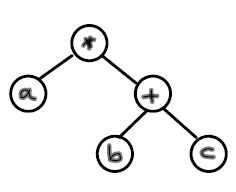
\includegraphics[scale=0.8]{bild2.png} \pause

entspricht dem arithmetischen Ausdruck:  $a \cdot (b + c)$
\end{frame}

%---
\begin{frame}[fragile]

Schnittstelle des ADT Baum:

\begin{tabular}{l l l }
 empty & : & liefert true, falls Baum leer \\
 left & : & liefert linken Teilbaum\\
 right & :  & liefert rechten Teilbaum\\ 
 value & : & liefert Wurzelelement \\
\end{tabular} 


In der Schnittstelle sind keine Methoden für das Wachstum des Baumes vorgesehen.  Wir nutzen dazu den Konstruktor.
\end{frame}

%---
\begin{frame}[fragile]
Implementation mittels verzeigerter Knoten 
 
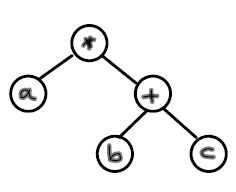
\includegraphics[scale=0.5]{bild2.png} 
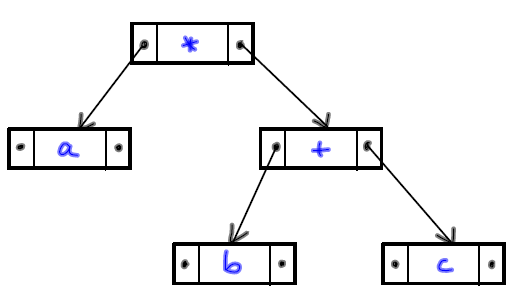
\includegraphics[scale=0.5]{bild4.png} ~~ 
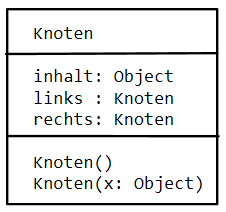
\includegraphics[scale=0.5]{bild4a.png}  


\begin{lstlisting}[mathescape=true]
class Knoten: $\pause$
    def __init__(self, x = None):
        self.inhalt = x
        self.links = None
        self.rechts = None
\end{lstlisting} 
\end{frame}

%----
\begin{frame}[fragile]
Der Baum hat zur internen Verwaltung nur einen Zeiger auf die wurzel.

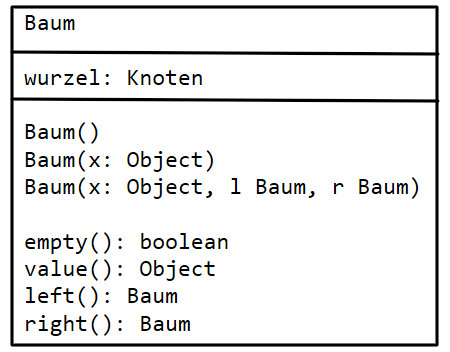
\includegraphics[scale=0.5]{bild5a.png}   

Mit \texttt{b = Baum()}
soll ein leerer Baum entstehen.   

\begin{minipage}[b]{5cm}
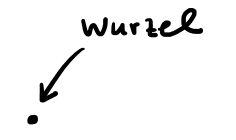
\includegraphics[scale=0.7]{bild5.png} 
\end{minipage}  
\begin{minipage}[b]{5cm}
\begin{lstlisting}
def __init__(self):  $\pause$
     self.wurzel = None
\end{lstlisting} 
\end{minipage} 

\end{frame}

\begin{frame}[fragile]
Ein Objekt x soll in der Wurzel des Baums gespeichert werden:

\begin{lstlisting}
b = Baum(x)
\end{lstlisting} 

\begin{minipage}[b]{5cm}
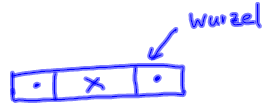
\includegraphics[scale=0.7]{bild6.png} 
\end{minipage}  
\begin{minipage}[b]{5cm}
\begin{lstlisting}
def __init__(self,$\pause$x = None): 
    self.wurzel = None
    if x is not None:
       self.wurzel = Knoten(x)
\end{lstlisting} 
\end{minipage} 

\end{frame}


%----
\begin{frame}[fragile]

Aus zwei Bäumen und einem Objekt x soll ein neuer Baum mit x in der Wurzel und den beiden Bäumen als linker und rechter Teilbaum geschaffen werden.
\begin{lstlisting}
b = Baum(x,l,r)
\end{lstlisting} 
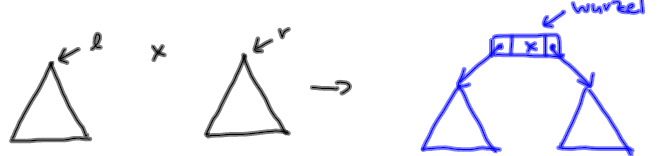
\includegraphics[scale=0.7]{bild7.png}  
\begin{lstlisting}
    def __init__(self,x = None,$\pause$l = None,r = None):
        self.wurzel = None
        if x is not None:
           self.wurzel = Knoten(x)
        if l is not None:
            self.wurzel.links = l.wurzel
        if r is not None:
            self.wurzel.rechts = r.wurzel
\end{lstlisting} 

\end{frame}

%---
\begin{frame}[fragile]
\begin{lstlisting}[basicstyle=\tiny]
class Baum:
    def __init__(self,x = None,l = None,r = None):
        self.wurzel = None
        if x is not None:
           self.wurzel = Knoten(x)
        if l is not None:
            self.wurzel.links = l.wurzel
        if r is not None:
            self.wurzel.rechts = r.wurzel
        
    def empty(self):   $\pause$
        return self.wurzel is None

    def value(self):   $\pause$
        if self.empty(): raise RuntimeError("Fehler: Baum ist leer")
        return self.wurzel.inhalt

    def left(self):   $\pause$
        if self.empty(): raise RuntimeError("Fehler: Baum ist leer")
        temp = Baum()
        temp.wurzel = self.wurzel.links
        return temp

    def right(self):   $\pause$
        if self.empty(): raise RuntimeError("Fehler: Baum ist leer")
        temp = Baum()
        temp.wurzel = self.wurzel.rechts
        return temp
\end{lstlisting} 
\end{frame}

%---
\begin{frame}[fragile]

Erzeuge folgenden Baum :


 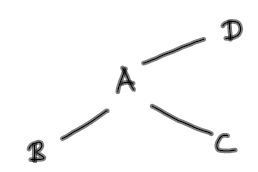
\includegraphics[scale=0.6]{bild8.png}  \pause

\begin{lstlisting}[mathescape=true]
a = Baum('a',Baum('b'),Baum('c'))
d = Baum('d',a,None)     
\end{lstlisting} 

\end{frame}

%---
\begin{frame}[fragile]

Einen Baum \textit{traversieren} bedeutet, jeden seiner Knoten besuchen.  

Verschiedene Reihenfolgen:  

\begin{itemize}
\item postorder - linker Sohn, rechter Sohn, Vater 
\item inorder -  linker Sohn, Vater, rechter Sohn
\item preorder -  Vater, linker Sohn, rechter Sohn 
\end{itemize} 

\begin{minipage}[b]{6cm}
 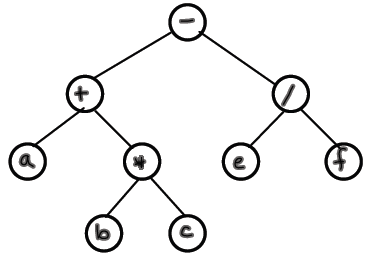
\includegraphics[scale=0.6]{bild9.png} 
\end{minipage}  \pause
\begin{minipage}[b]{5cm}
postorder: \pause a b c * + e f / - \\ 
inorder: \pause ~~ a + b * c - e / f  \\ 
preorder:  \pause ~ - + a * b c / e f 
\end{minipage} 
\end{frame}

%---
\begin{frame}[fragile]
Gib die Reihenfolge in postorder, inorder und preorder aus

 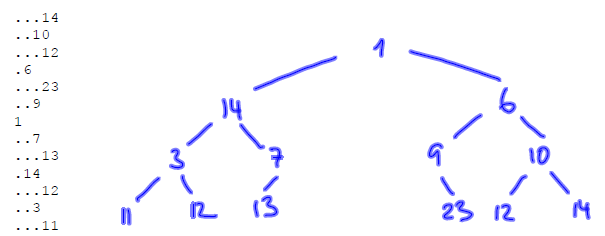
\includegraphics[scale=0.8]{bild10.png}  

postorder: \pause 11 12 3 13 7 14 23 9 12 14 10 6 1 \\ 
inorder: \pause ~~~11 3 12 14 13 7 1 9 23 6 12 10 14 \\ 
preorder: \pause ~ 1 14 3 11 12 7 13 6 9 23 10 12 14  


\end{frame}

%---
\begin{frame}[fragile]
Die richtige Reihenfolge zu programmieren, scheint nicht einfach zu sein.

Beispiel inorder:

 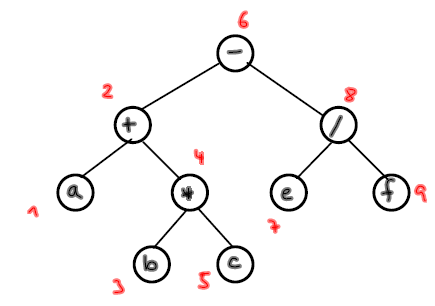
\includegraphics[scale=0.8]{bild11.png} 
\end{frame}

%---
\begin{frame}[fragile]
Ein Baum lässt sich mittels rekursiver Methoden traversieren.  

\begin{lstlisting}
def inorder(b):  $\pause$
    if b.empty(): return
    inorder(b.left())
    print(b.value(),end=" ")
    inorder(b.right())
\end{lstlisting} 

\begin{lstlisting}
def preorder(b): $\pause$
    if b.empty(): return 
    print(b.value(),end=" ")
    preorder(b.left())
    preorder(b.right())
\end{lstlisting} 

\begin{lstlisting}
def postorder(b):
    if b.empty(): return
    postorder(b.left())
    postorder(b.right())
    print(b.value(),end=" ")
\end{lstlisting} 

\end{frame}

%---
\begin{frame}[fragile]
\begin{minipage}[c]{7cm}
Die iterative Tiefensuche (preorder) wird mit einem Keller organisiert.  

Wir laufen nach links unten und legen die rechten Bäume, die uns unterwegs begegnen, in den Keller.  

 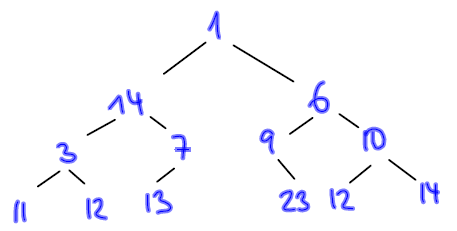
\includegraphics[scale=0.6]{bild12.png}   


\end{minipage}   \pause
\begin{minipage}[c]{4cm}
\begin{tabular}{l l}

Ausgabe & Keller \\ 
   & 1 \\  $\pause$
1 & 6 \\
14 & 7 6 \\
3 & 12 7 6\\
11 & 12 7 6 \\
12 & 7 6 \\
7 & 6 \\
13 & 6 \\
6 & 10 \\
9 & 23 10 \\
23 & 10 \\
10 & 14 \\
12 & 14 \\
14 & -
\end{tabular}
\end{minipage} 

\end{frame}

%---
\begin{frame}[fragile]
\begin{lstlisting}
def tiefenSuche(baum):  $\pause$
    k = Keller()
    if not baum.empty():
        k.push(baum)
    while not k.empty():
        b = k.top()
        k.pop()
        while not b.empty():
            print(b.value(),end=' ')
            if not b.right().empty():
                k.push(b.right())
            b = b.left()
    print()
\end{lstlisting} 
\end{frame}

%---
\begin{frame}[fragile]
\begin{minipage}[c]{7cm}
Bei der Breitensuche werden die Inhalte der Knoten ebenenweise ausgegeben. Sie wird mit einer Schlange organisiert.   

Wir reihen die linken und rechten Teilbäume in eine Schlange ein.  

 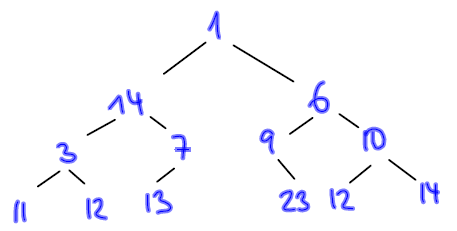
\includegraphics[scale=0.6]{bild12.png}   

\end{minipage} 
\begin{minipage}[c]{4cm}
\begin{tabular}{l l}
Ausgabe & Schlange \\  
 & 1 \\  $\pause$
1 & 14 6 \\
14 & 6 3 7 \\
6 & 3 7 9 10 \\
3 & 7 9 10 11 12 \\
7 & 9 10 11 12 13 \\
9 & 10 11 12 13 23  \\
10 & 11 12 13 23 12 14 \\
11 & 12 13 23 12 14 \\
12  & 13 23 12 14 \\
13 & 23 12 14 \\
23 &  12 14 \\
12 & 14 \\
14 & -
\end{tabular}
\end{minipage} 
\end{frame}

%---
\begin{frame}[fragile]
\begin{lstlisting}
def breitenSuche(baum):  $\pause$
    s = Schlange()
    if not baum.empty():
        s.enq(baum)
    while not s.empty():
        b = s.front()
        s.deq()
        print(b.value(),end=' ')
        if not b.left().empty():
            s.enq(b.left())
        if not b.right().empty():
            s.enq(b.right())
\end{lstlisting} 
\end{frame}


 \end{document}